\section{CUDA}

\subsection{Introduccion}

Una de las arquitectura analizadas en este trabajo es la arquitectura GPGPU desarrollada por \nvidia, conocida
como CUDA por las siglas en ingles de \textit{Compute Unified Device Architecture}.
CUDA surge naturalmente de la aplicaci\'on del hardware desarrollado gr\'aficos, pero aplicados al computo cient\'ifico.

Las placas de v\'ideo aparecen en 1978 con la introducci\'on de Intel del iSBX 275, permitiendo dibujar lineas,
arcos y bitmaps y comunicada por DMA al procesador principal. En 1985, la Commodore Amiga inclu\'ia un coprocesador
gr\'afico que podr\'ia ejecutar instrucciones independientemente del CPU, un paso importante en la separaci\'on
y especializaci\'on de las tareas. En la d\'ecada del 90, m\'ultiples
avances surgieron en la aceleraci\'on 2D para dibujar las interfaces gr\'aficas de los sistemas operativos,
y para mediados de la d\'ecada, muchos fabricantes estaban incursionando en las aceleradoras 3D como
add-ons a las placas gr\'aficas tradicionales 2D. A principios de la d\'ecada del 2000, se agregaron los
\textit{shaders} a las placas, peque\~nos programas independientes que corr\'ian nativo en el GPU,
y se pod\'ian encadenar entre si, uno por pixel en la pantalla.~\cite{CG} Este paralelismo es el desarrollo fundamental
que llevaba a las GPU a poder procesar operaciones gr\'aficas ordenes de magnitud m\'as r\'apidas que el CPU.

En el 2006, \nvidia introduce la arquitectura G80,
que es el primer GPU que deja de resolver \'unicamente problemas de gr\'aficos
para pasar a un motor gen\'erico donde cuenta con un set de instrucciones consistente para todos los
tipos de operaciones que realiza (geometria, vertex y pixel shaders).~\cite{cudaHandbook} Como subproducto de esto,
el GPU deja de tener pipelines especializados y pasa a tener procesadores sim\'etricos m\'as sencillos y m\'as
f\'aciles de construir. Esta arquitectura es la que se ha mantenido y mejorado en el tiempo, permitiendo
a las GPU escalar masivamente en procesadores simples, de un bajo clock de una disipaci\'on t\'ermica
manejable.

Los puntos fuertes de las GPGPU modernas consisten en poder atacar los problemas de paralelismo
de manera pseudo-explicita, y con esto poder escalar ``f\'acilmente'' si solamente se corre en una
placa mas r\'apida. ~\cite{} T\'ecnicamente, esta arquitectura cuenta con entre cientos y miles de procesadores
especializados en c\'alculo de punto flotante, procesando cada uno un \textit{thread} distinto pero
trabajando de manera sincr\'onica agrupados en bloques. Cada procesador a su vez cuenta con entre
64 a 256 registros~\cite{NvidiaFermi}~\cite{NvidiaKepler}, como porci\'on de un register file de 64kb.
Las placas cuentas con m\'ultiples niveles de cach\'e y memorias especializadas (subproducto de
su dise\~no fundamental para gr\'aficos). Estos no poseen instrucciones SIMD, ya que su dise\~no primario
esta basado en cambio, en SIMT (\textit{Single Instruction Multiple Thread}), las cuales se ejecutan en los
bloques sincr\'onicos de procesadores. De este modo, las placas modernas como la K40 alcanzan
poder de computo de 4.3 TFLOPs en c\'alculos de precisi\'on simple, 1.7 TFLOPs en precisi\'on doble y 288GB/seg de
transferencia, usando 2880 CUDA Cores.~\cite{NvidiaKeplerDatasheet} Para poner en escala la concentraci\'on
de poder de calculo, estas prestaciones har\'ian de una computadora usando solo dos de estas placas
la supercomputadora m\'as potente del mundo en Noviembre 2001.~\cite{Top500November2001}

\begin{figure}[htbp]
    \centering
    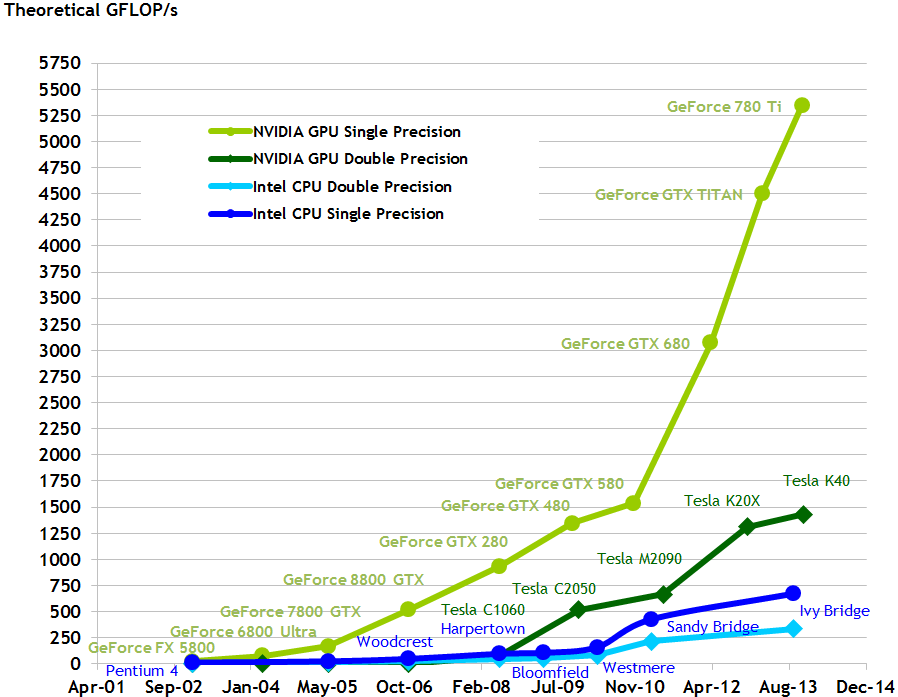
\includegraphics[width=\plotwidth]{images/cuda-gflops.png}
    \caption{Picos te\'oricos de performance en GFLOPS/s. Tomado de~\cite{cudaProgrammingGuide}.}
    \label{cuda-gflops}
\end{figure}

Para poder correr programas explotando la arquitectura CUDA, se deben escribir de manera que
el problema se pueda particionar usando el modelo de grilla de bloques de threads. Esto implica una
reescritura completa de los c\'odigos actuales en CPU y un cambio de paradigma importante, al
dejar de tener vectorizaci\'on, paralelizaci\'on autom\'atica y otras t\'ecnicas tradicionales
de optimizaci\'on en CPU. Sin embargo, este trabajo ha rendido sus frutos en muchos casos:
en los \'ultimos 6 a\~nos, la literatura de HPC con aplicaciones en GPU ha explotado con
desarrollos nuevos basados en la aceleraci\'on de algoritmos num\'ericos (su principal uso).
% ~\cite{meter refs a gpu montecarlos}
Adem\'as, no todas las aplicaciones deben reescribirse de manera completa. Con la introducci\'on
de las librer\'ias CuBLAS y CuFFT, se han buscado reemplazar con m\'inimos cambios las hist\'oricas
librer\'ias BLAS y FFTw, piedras fundamentales del computo HPC.~\cite{cublas}~\cite{cufft}

Nuevas soluciones para la portabilidad se siguen desarrollando: las librer\'ias como Thrust ~\cite{thrust},
OpenMP4.0 ~\cite{OpenMPspec} y OpenACC 2.0 ~\cite{OpenACCSpec} son herramientas que buscan hacer el
c\'odigo agn\'ostico al acelerador de computo que usen. Estas permiten definir las operaciones de
manera gen\'erica y dejan el trabajo pesado al compilador para que subdivida el problema de la manera
que el acelerador (CPU, GPU, MIC) necesite. Obviamente, los ajustes finos siempre quedan pendiente para
el programador especializado, pero estas herramientas representan un avance fundamental al uso
masivo de t\'ecnicas de paralelizaci\'on autom\'aticas, necesarias hoy d\'ia y potencialmente
imprescindibles en el futuro.

\subsection{Organizaci\'on de procesadores}

Los procesadores GPGPU dise\~nados por \nvidia han sido reorganizados a lo largo de su
existencia m\'ultiples veces pero mayormente tienen una distribuci\'on similar. Vamos a describir a continuaci\'on
la organizaci\'on definida en la arquitectura Fermi y luego analizaremos las diferencias con Kepler.

La arquitectura GPGPU se centran en el uso de una cantidad escable de procesadores
multithreaded denominados \textit{Streaming Multiprocessors (SMs)}. Un multiprocesador esta dise\~nado
para ejecutar cientos de threads concurrentemente, usando sus unidades aritm\'eticas llamadas \textit{Streaming
Processors (SPs)}. Para manejar esa cantidad de threads, se concibio una nueva entrada a la taxonom\'ia de Flynn,
SIMT (Single instruction, Multiple thread). Las instrucciones se encadenan para aprovechar el paralelismo
a nivel instrucci\'on (ILP) dentro de un mismo threads, y funcionando en conjunto con el paralelismo
a nivel de thread, usado de manera extensa a trav\'es del multithreading por hardware. Todas las instrucciones
son ejecutadas en orden y no hay predicci\'on de saltos ni ejecuci\'on especulativa, todo se ejecuta solamente
cuando se lo necesita. ~\cite{CudaOverview}

\begin{figure}[htbp]
    \centering
    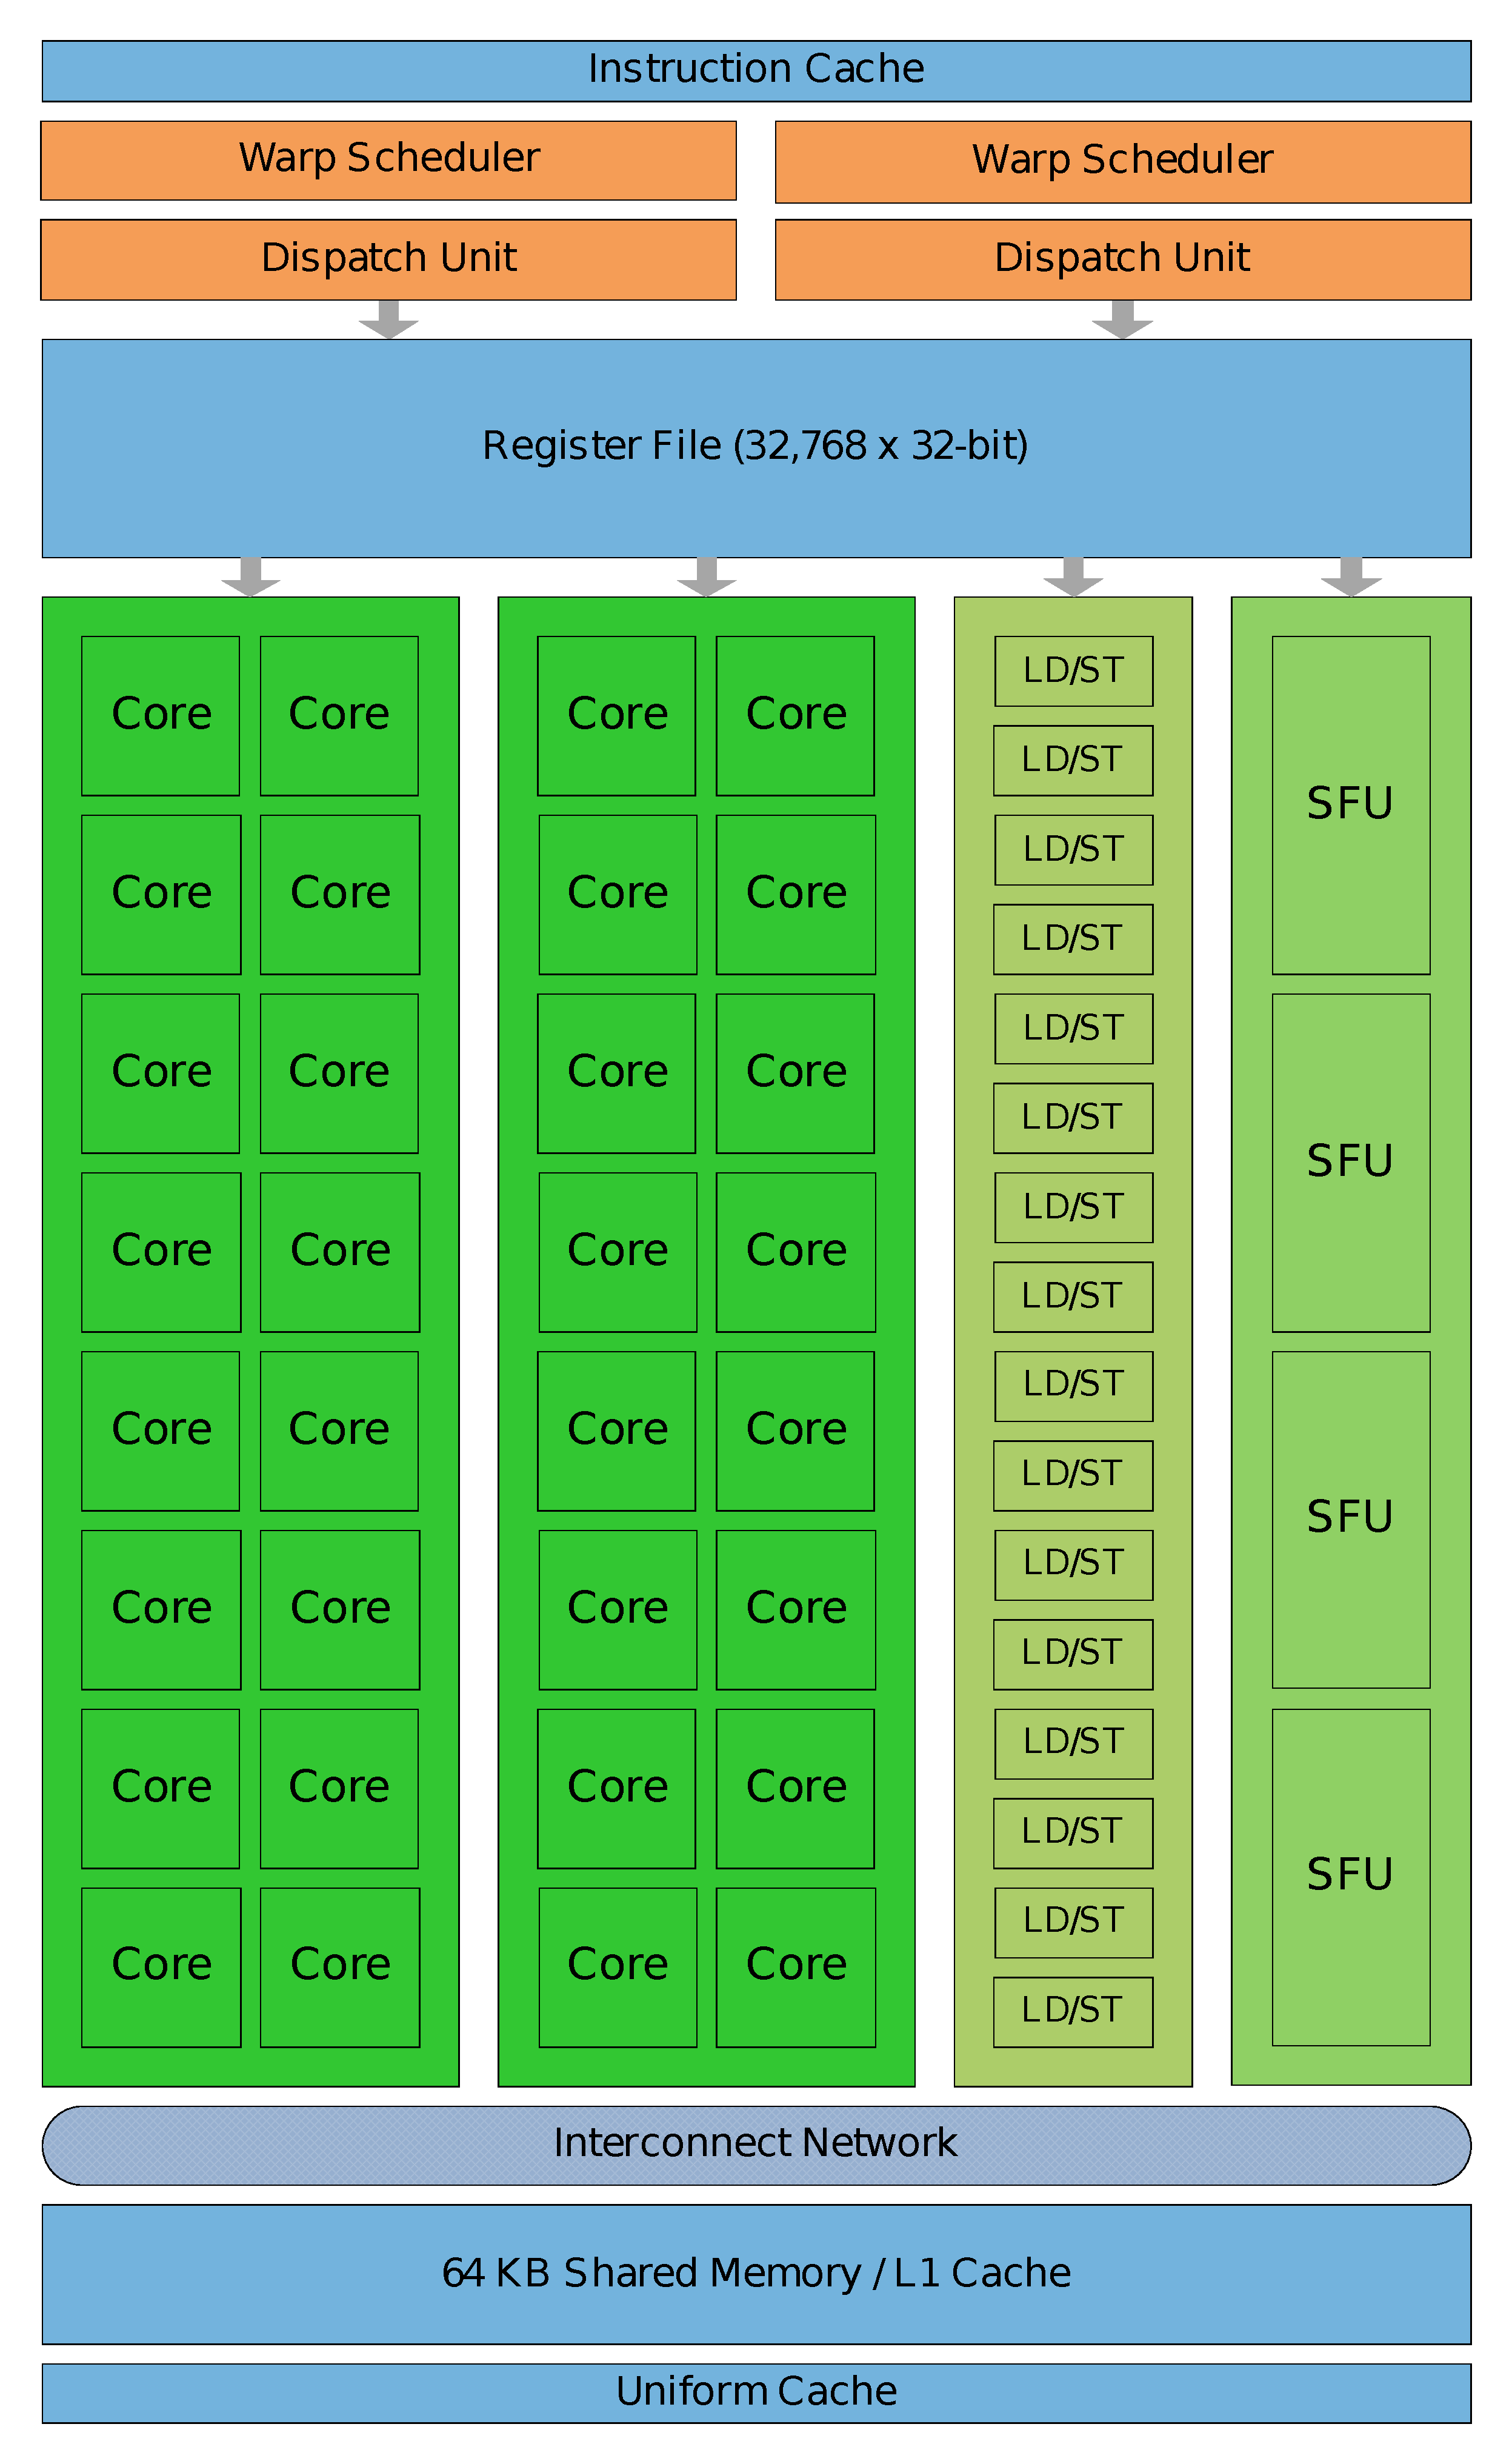
\includegraphics[width=\plotwidth]{images/fermi-sm.pdf}
    \caption{Diagrama de bloques del SM de GF100 Fermi. Tomado de~\cite{NvidiaFermi}.}
    \label{fermi_sm}
\end{figure}

Los SM son unidades completas de ejecuci\'on. Estos tienen 32 SPs interconectados entre si, que operan sobre
un register file com\'un a todos. Los SM cuentan adicionalmente con m\'ultiples unidades de Load/Store,
que permiten realizar accesos a memoria independientes. Existen 4 unidades de SFU (\textit{Special Function
Unit}) por SM, para realizar r\'apidamente operaciones matem\'aticas trascendentales (trigonom\'etricas, potencias,
ra\'ices, etc.). Cada SM ejecuta simult\'aneamente una cantidad fija de threads, llamado \textit{warp}
con cada uno de estos corriendo en un SP. Las unidades de despacho de warps se encargan de mantener registro de que
threads est\'an disponibles para correr en un momento dado y permiten realizar cambios de contexto por hardware
eficientemente ($<25 \mu$s)~\cite{PattersonFermi}. Con esto, se pueden ejecutar
concurrentemente dos warps distintos para esconder la latencia de las operaciones. En precisi\'on doble,
esto no se puede, as\'i que hay solamente un warp corriendo a la vez.

Un SM cuenta con una memoria com\'un de 64kb que se puede usar de forma autom\'atica tanto como memoria
compartida com\'un a todos los threads como cach\'e L1 para todos los accesos a memoria.

\begin{figure}[htbp]
    \centering
    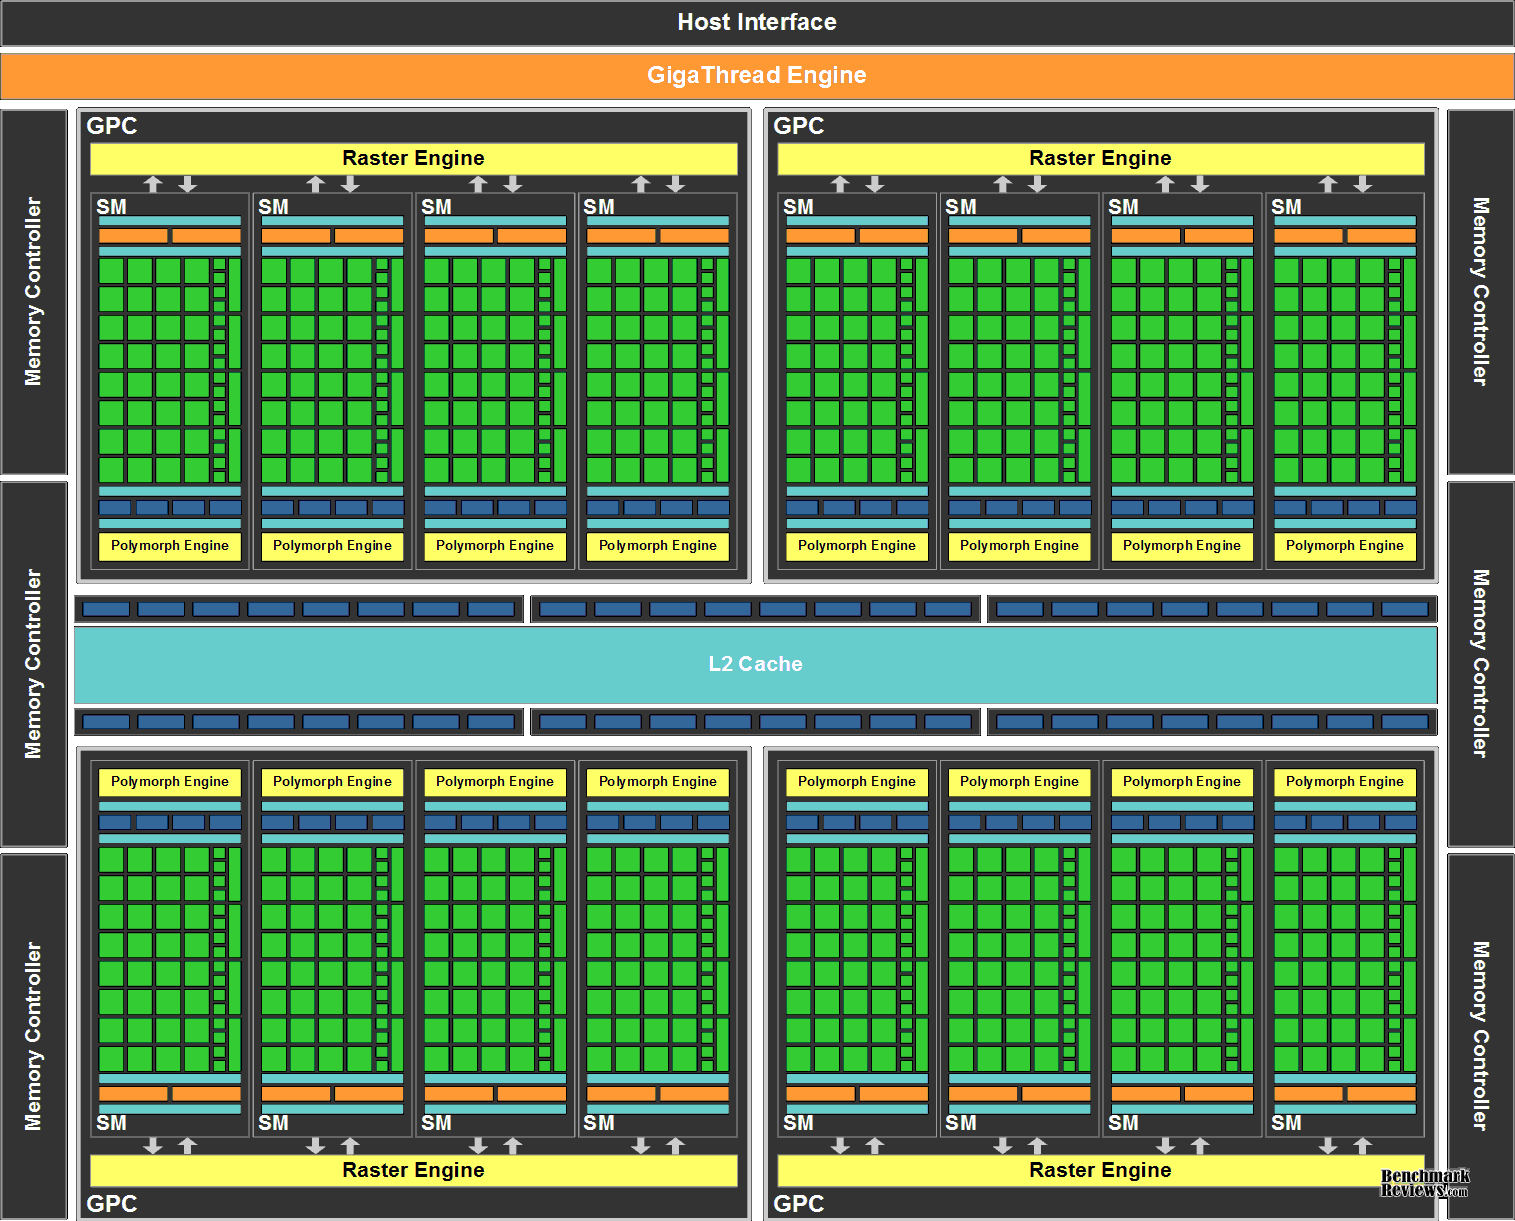
\includegraphics[width=\plotwidth]{images/fermi-gpu-block.png}
    \caption{Diagrama de bloques de GF100 Fermi. Tomado de~\cite{NvidiaFermi}.}
    \label{fermi_gpu_block}
\end{figure}


Por motivos de como funciona un pipeline gr\'afico, los SM se agrupan de 4, en un GPC (\textit{Graphics
Processing Cluster}). Cada GPC se encarga de ejecutar los distintos pasos del pipeline gr\'afico,
cargando a los SM con las tareas que tienen que realizar para rasterizar (es decir, convertir los
gr\'aficos vectorialmente definidos en gr\'aficos renderizados). En aplicaciones de CUDA, estos pasos
no importan, puesto que se trata cada SM independientemente por software.

Todos los accesos a memoria global (la memoria off-chip del dispositivo) se realizan a trav\'es de la memoria
L1 de cada SM, y a trav\'es de la L2 del todo el procesador. Esta L2 consiste de 6 bancos de 128Kb, compartidas.
Estas cach\'e son write-through y se comunican de manera directa tanto con la DRAM propia de la placa como
con el bus PCI Express por el cual pueden comunicarse dos placas entre si, sin pasar por CPU.

En Fermi no se pueden ejecutar simult\'aneamente instrucciones de precisi\'on doble y simple, y como
las de doble requieren ambos pipelines, suelen disminuir considerablemente el aprovechamiento
de los cores. En Kepler, al usar 4 unidades de despacho de warp, puede elegir una mejor
combinaci\'on para poder ejecutar simult\'aneamente instrucciones que no dependan de las mismas
unidades funcionales en el pipeline. ~\cite{NvidiaKepler}

Como estos procesadores implementan el est\'andar IEEE754-2008, cuentan con precisi\'on simple y
doble correcta, por lo cual dentro de las operaciones nativas, cuentan con instrucciones FMA
(Fused multiply-add) que no pierden precisi\'on en etapas intermedias de redondeo.



%El c\'odigo escrito para CUDA se puede compilar a dos targets distintos; uno es
%el codigo binario nativo de la placa target donde se va a correr y el otro es un
%codigo intermedio, llamado c\'odigo PTX, que se JIT compila por el driver CUDA
%antes de enviar a la placa, de modo que sea portable entre placas y arquitecturas
%(retrocompatibles).

%Cuando se lanza un kernel de ejecuci\'on, este c\'odigo binario se carga en la DRAM propia
%de la placa. Este codigo va a ser ejecutado por todos los bloques que se hayan definido cuando
%se lanz\'o el kernel. El ``Thread Engine'' del GPGPU se encarga de repartir los bloques a los
%SM (Streaming Multiprocessors). Cada SM luego va a ejecutar de a grupos de 32 threads, cada uno
%de ellos corriendo sobre un SP (Streaming Processor). A traves de sus 2 o 4 unidades de dispatch de warp
%(de acuerdo a la generaci\'on de los chips), el SM puede dinamicamente cambiar el warp que se esta ejecutando en sus SP,
%escondiendo la latencia de los stalls de pipelines forzosos para la ejecucion de instrucciones de multiples clocks.
%Estos threads a su vez obtienen sus registros de un register file com\'un a todos los SP. Un scoreboard
%es mantenido por cada dispatcher de warps para poder determinar que threads estan listos para correr. En Kepler
%este scoreboard es simplificado ya que las latencias de las operaciones matem\'aticas es conocido, por
%lo cual se puede reemplazar por contadores m\'as sencillos. ~\cite{NvidiaKepler}
%Como el c\'odigo se ejecuta de manera sincr\'onica entre todos los threads del warp, las instrucciones
%condicionales proveen un problema para esta arquitectura. Como las distintas ramas del condicional
%son instrucciones excluyentes, no las deben ejecutar todos los threads simultaneamentes. El procesador
%deshabilitaba los cores que manejaban los threads de las ramas que no se ejecutaban del
%condicional~\cite{NvidiaTesla}. Para disminuir la cantidad de instrucciones de condicionales
%que se ejecutan, se cuenta con ~\cite{NvidiaFermi} predicaci\'on en todas las instrucciones de la ISA.


\subsection{Organizaci\'on de la memoria}

%La arquitectura CUDA esta enfocada a procesamiento de grandes cantidades de datos
%de puntos flotante. El procesador GPGPU cuenta con cientos de ALU sincronizadas
%por bloques, permitiendo un paralelismo adaptativo a distintos problemas.
%
%El procesamiento GPGPU es similar al procesamiento vectorial
%realizado por las supercomputadoras Cray y IBM que surgio en los 1960's, pero
%en vez de usar VLIW para procesamiento masivo, CUDA usa multiples hilos de ejecuci\'on
%que trabajan simultaneamente sobre los datos.
%El procesamiento consiste en un funcionamiento hibrido entre compilador y procesador. Se determina
%un conjunto de elementos a procesar y se elije de manera explicita una manera de particionar el
%problema a la hora de ser enviado para procesado a la placa.
%
%Para realizar el computo, esta arquitectura cuenta a su vez con multiples clases de memorias
%que se adaptan de maneras diferentes a los distintos procesos. Estas incluyen:
La memoria de la GPGPU es uno de los puntos cruciales de esta arquitectura. Esta se subdivide
entre memorias on-chip y memorias on-board, de acuerdo a su ubicaci\'on y tiempos de acceso.

Las memorias se subdividen en 4 categor\'ias distintas:

\begin{itemize}
  \item Registros
  \item Memoria global
  \item Memoria local
  \item Memoria compartida
\end{itemize}

Los registros son la unidad b\'asica de almacenamiento de los threads de ejecuci\'on.
Cada thread de ejecuci\'on cuenta con una cantidad limitada de registros de punto flotante de
32 bits con latencia de un par de ciclos de clock. A su vez, existen una cantidad finita de
registros totales que cuenta un chip (oscilan entre 16.535 y 65.535 registros).

La memoria global es la memoria principal fuera del chip del GPGPU. Esta es de gran tama\~no (de
entre 2Gb y 12Gb) y es compartida por todos los SM de la GPGPU y los CPU que integran el
sistema. Es decir, tanto los GPGPU y los CPU pueden invocar las funciones del runtime CUDA
para poder transferir datos entre la placa y la memoria RAM. La latencia de acceso a la memoria global
es de cientos de ciclos~\cite{Demystifying}, sumamente lenta en comparaci\'on con el procesador.
La memoria global tambi\'en puede ser mapeada, o \textit{pinneada}. Esto quiere decir que va a existir
una copia de esa reserva de memoria en la placa en la memoria principal del procesador. El driver
de CUDA va a mantener la consistencia entre ambas de manera as\'incrona, evitando la necesidad de hacer
copias de memoria explicitas. No es ilimitada la cantidad de memoria mapeada posible, por lo que
es importante saber elegir que elementos van a ir en esta.

La memoria compartida, o \textit{shared}, es una memoria que es visible para todos los threads dentro
de un mismo SM. Cada thread puede escribir en cualquier parte de la memoria compartida dentro de su bloque y
puede ser le\'ido por cualquier otro thread de este. Es una memoria muy r\'apida, on-chip, y
que tarda aproximadamente 40 ciclos de acceso.~\cite{Demystifying} Esta memoria es compartida con la cach\'e
L1, de capacidad de entre 16Kb y 64kb configurable por software. Esta memoria se encuentra dividida
en 32 bancos de 4 bytes de tama\~no, permitiendo que cada uno de los 32 threads acceda independientemente
a un float. Si hubiera conflicto, los accesos a ese banco se serializar\'ian, aumentando la latencia
de la llamada.~\cite{farberCuda}

La memoria local es una memoria propia de cada thread, y se encuentra almacenada dentro de la
memoria global. Esta memoria es definida autom\'aticamente por el compilador y sirve como \'area de \textit{spilling}
de registros cuando se acaban. Cuenta con las mismas desventajas que la memoria global, incluyendo
su tiempo de acceso.

Adicionalmente, la GPGPU cuenta con m\'ultiples niveles de memorias cach\'e para poder aminorar el hecho
de que el principal cuello de botella del computo es la latencia en los accesos a memoria global.
Estas se dividen en tres:

\begin{itemize}
  \item Cach\'e L1
  \item Cach\'e L2
  \item Cach\'e de textura
\end{itemize}

La cach\'e L1 es dedicada por SM. Esta cach\'e fue introducida en Fermi y su dise\~no hace que
tambi\'en esta dedicada a la memoria compartida, por lo que es posible en tiempo de ejecuci\'on
darle directivas a la GPGPU que asigne m\'as memoria cach\'e o m\'as memoria compartida,
permitiendo a los bloques tener mayores espacios de memorias compartidas o mayores hit rate de caches.

La cach\'e L2 es com\'un a todos los SM de la GPGPU, donde, a partir de Fermi en \nvidia, todos
los accesos de lectura y escritura a memoria global y textura pasan a trav\'es de esta. ~\cite{NvidiaFermi}

La cach\'e de textura es una cach\'e sobre la memoria global que presenta no solo localidad espacial,
como la mayor\'ia de las caches de procesadores normales (es decir, dato-1, dato, dato+1, etc.), sino que se le
puede agregar el concepto de dimensiones, para poder modelar datos en mas de una dimensi\'on.
Esto se adapta de muy bien a los problemas de gr\'aficos en el 2D y 3D, por lo tanto se convierte
en una herramienta clave a la hora de minimizar los accesos a matrices
no solo por filas sino por columnas. Esta cach\'e se debe definir en momento de compilaci\'on en
en el c\'odigo, ya que tiene limites espaciales (necesarios para poder definir \'areas de memoria
sobre la cual operar) y a su vez se debe acceder a los datos subyacentes a trav\'es de funciones especificas. Una caracter\'istica adicional
de esta cach\'e es que como necesita resolver estos accesos no convencionales a la memoria, cuenta
con una unidad propia de resoluci\'on de direcciones. Esta unidad tiene limitantes a cuanto podemos
exigirle, ya que no posee un ancho de banda suficiente como para resolver todos los
accesos a memoria globales podr\'ia servir, as\'i que hay que usarla juiciosamente.

\begin{figure}[htbp]
    \centering
    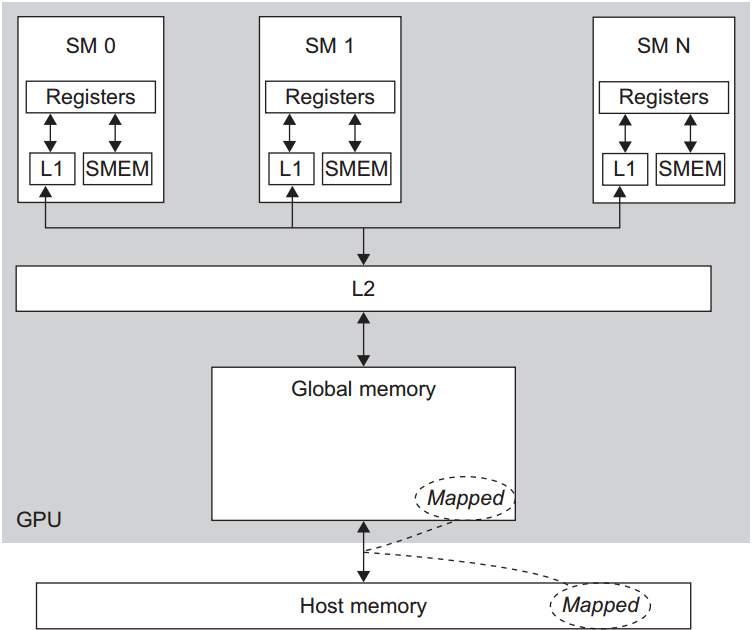
\includegraphics[width=250px]{images/cuda-memories.png}
    \caption{Jerarqu\'ia de memorias en GPU. Tomado de~\cite{farberCuda}.}
    \label{fig:cuda-memories}
\end{figure}

\subsection{Esquema de paralelismo}
Al ser una arquitectura masivamente paralela desde su concepci\'on, CUDA presenta varios niveles de paralelismo, para
agrupar l\'ogicamente el computo y poder dividir f\'isicamente su distribuci\'on. Los principales son:
\begin{itemize}
  \item Bloques de threads
  \item Grilla de bloques
  \item Streams
  \item M\'ultiples placas
\end{itemize}

El paralelismo a nivel de bloque instancia una cantidad de threads, subdivididos l\'ogicamente en 1D, 2D o 3D.
Los threads internamente se agrupan de a 32 threads (un \textit{warp}).
Cada uno de estos threads va a contar su propio threadId y con el mismo blockId, identific\'andolos un\'ivocamente.
Estos threads van a correr simult\'aneamente en el mismo SM y van a ser puestos y sacados de ejecuci\'on de a un warp
din\'amicamente por el scheduler de hardware que cuenta cada SM. Para compartir informaci\'on entre
ellos, se puede utilizar la memoria shared o las instrucciones de comunicaci\'on de threads intrawarp.

El paralelismo a nivel de grilla determina una matriz de bloques de ejecuci\'on que partici\'on
el dominio del problema. El GigaThread Scheduler va a ejecutar cada bloque en un SM hasta
el final de la ejecuci\'on de todos los threads de este. Los bloques entre si no comparten informaci\'on
sino a trav\'es de la memoria global. Como no se garantiza ning\'un orden de ejecuci\'on no se puede
confiar en sincronizar entre si, ya que si hay m\'as bloques que SM y no hay pre-emption en los SM,
puede haber deadlock.

El paralelismo de stream es una herramienta empleada para hacer trabajos concurrentes usando una
sola placa. Esta t\'ecnica permite que m\'ultiples kerneles o copias de memoria independientes est\'en
encolados, para que el driver pueda schedulearlas simult\'aneamente si se est\'an subutilizando
los recursos de forma de minimizar tiempo ocioso del dispositivo. Los streams permiten kernels
concurrentes pero cuentan con importantes restricciones que generan sincronizaci\'on impl\'icita,
lo cual hay que tener presente si se desea mantener el trabajo de forma paralela.

El paralelismo a nivel de placa consiste en poder distribuir la carga del problema entre distintas
GPGPU dispuestas en un mismo sistema compartiendo una memoria RAM com\'un como si fuera un software
multithreaded tradicional. CUDA no cuenta con un modelo impl\'icito de paralelismo entre distintas placas,
pero es posible hacerlo manualmente eligiendo de manera explicita que dispositivo usar. Las placas
se pueden comunicar as\'incronamente entre si, tanto accediendo a las memorias globales de cada una
como ejecutando c\'odigo remotamente. En las versiones modernas del driver de CUDA, tambi\'en pueden
directamente comunicarse las placas entre si a trav\'es de la red, permitiendo escalar multinodo f\'acilmente.

Los algoritmos de GPGPU deben considerar todos estos niveles de paralelismo para poder maximizar la
performance, empleando as\'i todos los recursos con los que cuentan estas arquitecturas.

\subsection{Diferencias entre Tesla, Fermi, Kepler}

Hasta ahora enunciamos la arquitectura vista desde el punto de vista Fermi, la segunda
arquitectura GPGPU dise\~nada por \nvidia . Fermi es la evoluci\'on de Tesla,
construida para desacoplar a\'un mas los conceptos de gr\'aficos de modo de hacerla
un procesador m\'as escalable y de prop\'osito general.


\begin{table}[h]
  \begin{tabular}{@{}llll@{}}
  \toprule
  Caracter\'isticas        & Tesla (GT200)   & Fermi (GF100)   & Kepler (GK110)   \\ \midrule
  A\~no introducci\'on     & 2006            & 2010            & 2012             \\
  Transistores             & 1400 millones   & 3000 millones   & 3500 millones    \\
  Tecnolog\'ia fabricaci\'on & 65 nm           & 40 nm           & 28 nm            \\
  SMs                      & 30              & 16              & 15               \\
  SP / SM                  & 8               & 32              & 192              \\
  Cach\'e L1               & -               & 16 - 48Kb       & 16 - 32 - 48Kb   \\
  Cach\'e L2               & -               & 768Kb           & 1536Kb           \\
  Memoria Shared/SM      & 16Kb            & 16 - 48Kb       & 16 - 32 - 48Kb   \\
  Registros/Thread         & 63              & 63              & 255              \\
  Pico Precisi\'on Simple    & 240 MAD / clock & 512 FMA / clock & 2880 FMA / clock \\
  Pico GFLOPS Simple       & 933             & 1345            & 3977             \\
  GFLOPS/Watt              & 3.95            & 5.38            & 15.9             \\ \bottomrule
  \end{tabular}
\caption{Tabla comparativa de las caracter\'isticas mas prominentes de las tres arquitecturas de CUDA.}
\label{tab:CudaGenerations}
\end{table}

En la tabla \ref{tab:CudaGenerations} vemos una comparaci\'on de las recursos que est\'an m\'as directamente
relacionadas a la performance de un dispositivo GPGPU. Se puede apreciar como muchos recursos
crecieron dr\'asticamente gracias a las tecnolog\'ias de fabricaci\'on, que permitieron aumentar la
cantidad de transistores. Tambi\'en podemos comprobar que, a diferencia de los CPU, las arquitecturas GPGPU
decidieron utilizar esos nuevos transistores disponibles para mas n\'ucleos de procesamiento, en vez
de dedicarlas a aumentar las memorias cach\'e, que crecieron m\'inimamente (comparando contra las caches de CPU).

Una de las diferencias mas notables entre Tesla y Fermi es la presencia de FMA (\textit{Fused Multiply-Add})
contra el MAD (\textit{Multiply - Add}). El MAD realiza la multiplicaci\'on y la acumulaci\'on
en dos pasos (pero m\'as r\'apidos que hacerlos independientemente por tener hardware dedicado en los SP)
debe redondear entre los pasos, perdiendo precisi\'on y haciendo que respete plenamente el IEEE754-2008. El FMA,
en cambio, lo hace en una sola operaci\'on, y sin redondeos intermedios.

La m\'etrica usada por \nvidia para publicitar la performance de estos dispositivos y poder
compararlos entre si, y contra CPU, son los GFLOPS. Esta unidad mide cuantas operaciones de punto
flotante de precisi\'on simple se pueden realizar por segundo. Esta unidad es utilizada tambi\'en
por los clusters en el ranking TOP500, donde se ordenan de acuerdo al pico de performance medido. No solo
es notable como se cuadruplico la performance (te\'orica) en solamente 6 a\~nos (algo inalcanzable para
los CPU modernos) sino que a\'un mas notorio es como mejoro la performance por Watt. Esto
tambi\'en se ve en que Kepler tiene menos SM que Fermi o Tesla, pero son mucho mas poderosos y
eficientes. La tecnolog\'ia de fabricaci\'on ha ayudado a la disminuci\'on del consumo, un
problema que acechaba a los dise\~nos Fermi, ya que sus consumos superiores a 200W por
dispositivo los hac\'ian muy dif\'iciles de refrigerar incluso en clusters de HPC. Se puede
notar la estrategia de mercado de \nvidia de introducirse en las supercomputadoras de todo
el mundo, donde el consumo y la refrigeraci\'on son factores limitantes (mucho m\'as aun que,
por ejemplo, computadoras de escritorio).

\subsection{CUDA, Herramientas de desarrollo, profiling, exploraci\'on}

Para soportar una arquitectura masivamente paralela, se debe usar una ISA
(\textit{Instruction Set Architecture}) dise\~nada especialmente para el problema. Esta ISA, conocida como PTX,
debe poder soportar conceptos fundamentales del computo GPGPU: grandes cantidades de registros,
operaciones en punto flotante de precisi\'on simple y doble y fused multiply-add. Adem\'as,
el c\'odigo compilado para GPGPU debe ser agn\'ostico al dispositivo que lo va a correr, por
lo cual la paralelizaci\'on no debe estar demasiado atada a este, sino que el dispatching
lo debe poder determinar el driver de la placa en tiempo de ejecuci\'on.  Un \'ultimo
requerimiento clave de esta ISA es que debe poder soportar poder realizar ajustes manuales,
para poder construir partes claves de ciertas librer\'ias frecuentemente usadas (como las BLAS)~\cite{NvidiaFermi}.

El lenguaje que desarrollo \nvidia para poder programar estos dispositivos a un nivel m\'as alto
que el assembler especifico del procesador es CUDA. Este lenguaje es una extensi\'on de C++, con ciertas
features agregadas para poder expresar la subdivisi\'on de los kernels en threads y bloques, junto
con poder especificar que variables y funciones van a ejecutarse en el GPGPU y en el CPU. Una caracter\'istica
de CUDA es que todas las llamadas a los kernels de ejecuci\'on son asincr\'onicas, por lo que es relativamente
sencillo solapar c\'odigo en GPU y CPU. A su vez se cuenta con m\'ultiples funciones opcionales, con distinta
granularidad, que permiten esperar a que todas las llamadas as\'incronas a GPU finalicen, agregando determinismo
en forma de barreras al lenguaje.

El c\'odigo CUDA compila usando \texttt{nvcc}, una variante del \texttt{GNU gcc} que se
encarga de generar el c\'odigo PTX para las funciones marcadas como que se van a ejecutar
en los GPGPU. Este c\'odigo objeto despu\'es se linkea normalmente con el resto del c\'odigo que corre en CPU
y se genera un binario ejecutable.

\nvidia, ademas, provee herramientas de profiling para explorar como se est\'an utilizando los
recursos durante la ejecuci\'on. Estas son esenciales para optimizar, puesto que los limitantes
de GPU son sumamente distintos a los de CPU, presentando dificultades incluso para programadores
experimentados. Las herramientas de profiling no solo muestran runtime, sino que sirven para
ver donde hay accesos a memoria excesivos, puntos de sincronizaci\'on costosos, limitantes
en los registros y como se superponen las llamadas asincr\'onicas.

El uso de todas estas herramientas fue vital para poder entender como funciona la arquitectura por dentro,
como medir performance y utilizaci\'on y como nuestros cambios impactan en las distintas generaciones
de dispositivos.

\subsection{Requerimientos de un problema para GPGPU}
Dada la organizaci\'on de un procesador GPGPU, es posible ver como esta apuntado a ejecutar
algoritmos de dominios muy espec\'ificos. Un problema debe exhibir al menos las siguientes
caracter\'isticas para que valga la pena pensar en correrlo para GPGPU.
\begin{enumerate}
  \item \label{req:paralelo} El problema debe tener una gran parte paralelizable.
  \item \label{req:float} El problema debe consistir mayormente de operaciones num\'ericas de punto flotante.
  \item \label{req:matrix} El problema debe poder ser modelado mayormente en arreglos o matrices.
  \item \label{req:transf} El tiempo de computo debe ser muy superior al tiempo de transferencia de datos.
\end{enumerate}

Item \ref{req:paralelo} se refiere a que debe existir alguna forma de partir el problema
en subproblemas que puedan realizarse simult\'aneamente, sin que haya dependencias de
resultados entre si. Si el problema requiere partes seriales, lo ideal es que se las
pueda concebir las partes paralelas sean etapas de un pipeline de procesos, donde
cada una de estas exhiban caracter\'isticas fuertemente paralelas. Como las arquitecturas
masivamente paralelas tienen como desventaja una menor eficiencia por core, si el
problema no se puede dividir para maximizar la ocupaci\'on de todos los cores disponibles,
va a ser muy dif\'icil superar en eficiencia a los procesadores seriales.

Item \ref{req:float} habla de que el m\'etodo de resoluci\'on de los problemas debe
consistir del uso de m\'etodos num\'ericos. El set de instrucciones de las arquitecturas
de GPGPU est\'an fuertemente influenciados por las aplicaciones 3D que las impulsaron
en un principio. Estas consisten mayormente de transformaciones de \'algebra lineal
para modelar luces, hacer renders o mover puntos de vistas. Todos estos problemas
son inherentemente de punto flotante, por lo cual el set de instrucciones, las ALUs
internas y los registros est\'an optimizados para este caso de uso. Las operaciones
en n\'umeros enteros no son el fuerte de esta arquitectura y suelen ser realizados
m\'as eficientemente por procesadores de prop\'osito general.

Item \ref{req:matrix} menciona que los problemas que mejor se pueden tratar en esta
arquitectura se pueden representar como operaciones entre arreglos o matrices de
dos, tres o cuatro dimensiones. Las estructuras de datos que no est\'an secuenciales
en memoria pueden incurrir en m\'ultiples accesos a esta para recorrerlas, y en las
arquitecturas GPGPU son estos los que generan el mayor cuello de botella. Ademas,
suelen ser dif\'iciles de paralelizar en m\'ultiples subproblemas. Tener como par\'ametros de
entrada matrices o arreglos que se puedan partir f\'acilmente incurre en m\'inimos
overheads de computo y permite aprovechar mejor las memorias caches y las herramientas de
prefetching que brinda la arquitectura.

Item \ref{req:transf} ataca uno de los puntos cr\'iticos de esta arquitectura. Para poder
operar con datos, se requiere que estos est\'en en la memoria de la placa, no la memoria
de prop\'osito general de la computadora. Esto quiere decir, que se deben hacer copias
explicitas entre las memorias, ya que ambas tienen espacios de direcciones independentistas.
Esta copia se realiza a trav\'es de buses que, a pesar de tener un enorme throughput de
datos, tambi\'en tienen una gran latencia (orden de milisegundos). Por lo tanto, para minimizar
el tiempo de ejecuci\'on de un programa usando las GPGPU, se debe considerar tambi\'en el
tiempo de transferencia de datos a la hora de determinar si el beneficio de computar en
menor tiempo lo justifica. Las nuevas versiones de CUDA buscan brindar nuevas herramientas
para simplificar este requerimiento, proveyendo espacio de direccionamiento \'unico y
memoria unificada ~\cite{farberCuda}, pero siguen siendo copias de memoria a trav\'es de los
buses (aunque asincr\'onicas).

Estas caracter\'isticas limitan enormemente la clase de problemas que una GPGPU puede
afrontar, y suelen ser una buena heur\'istica para determinar de antemano si vale la pena
invertir el tiempo necesario de la implementaci\'on y ajuste fino.


\subsection{Diferencia entre CPU y GPU - Procesadores especulativos}
Hasta ahora, solo se consideraron a los GPGPU de forma aislada, viendo las prestaciones del hardware y un m\'inimo
de como se escriben los programas para esta arquitectura. La esencia de GPGPU se puede apreciar mejor
compar\'andola contra los motivos de la evoluci\'on de CPU, y los problemas que se fueron enfrentando
los dise\~nos siguiendo la historia de los componentes que fueron apareciendo en estos. Esto se vio
en la tabla \ref{tbl:historia-cpu}, que detalla algunos de los eventos m\'as importantes que aceleraron
la performance de los CPU.

Lo importante ac\'a es observar el patr\'on: ``no desechar algo que pudi\'eramos necesitar pronto'',
``intentar predecir el futuro de los condicionales'', ``intentar correr m\'ultiples instrucciones a la vez
porque puede llegar a bloquear en alguna de ellas.''

Todos estos problemas han convertido al CPU en un dispositivo que gira alrededor de la especulaci\'on,
de los valores futuros que pueden tener las ejecuciones, del probable reuso de datos.
En un CPU moderno (por ej. Intel Xeon E7-8800~\cite{XeonE78800Spec}) las unidades que verdaderamente realizan las operaciones l\'ogico-aritm\'eticas,
las ALU, son muy pocas en comparaci\'on con la cantidad de dispositivos de soporte que est\'an
sobre el silicio del CPU.

En contraste, los dispositivos GPGPU son verdaderos procesadores de computo masivo. Est\'an dise\~nadas para
resolver constantemente operaciones muy bien definidas (instrucciones de punto flotante en su mayor\'ia).
Comparativamente con un CPU, las ALU de las GPU son bastante pobres y lentas. No funcionan a las mismas
velocidades de clock (rara vez superan 1.1Ghz) y sus SP deben estar sincronizados entre si. Pero la gran ventaja esta en la cantidad.
Un CPU cuenta con pocas ALU por core, dependiendo de la cantidad de cores y del tama\~no de sus operaciones SIMD
(alrededor de 16 cores por die de x86 es el tope de linea ofrecido actualmente, procesando de a 32 bytes simult\'aneamente).
Un GPU cuenta con miles de ALUs en total (m\'as de 2500 CUDA Cores en Tesla K20). El dise\~no de esta
arquitecturas concibe la escalabilidad cuantitativa de los unidades de computo como la caracter\'istica esencial a tener,
tanto por su \'enfasis fundamental, las aplicaciones gr\'aficas, como para su aspecto de coprocesador num\'erico
de prop\'osito general.

Por contrapartida, los GPU disponen de pocas unidades de soporte del procesamiento. Estos no disponen pipelines
especulativos, el tama\~no de las caches est\'an a ordenes de magnitud de las de CPU, la latencia a las memorias
principales de la GPU est\'an a centenas de clocks de distancia, etc. La arquitectura asume que siempre va a tener m\'as trabajo
para hacer, por lo cual en vez de intentar solucionar los pitfalls de un grupo de threads, directamente
los reschedulea para m\'as adelante y continua procesando otro warp de threads. Se puede notar que durante del
dise\~no de la arquitectura GPGPU buscaron resolver el problema del computo masivo pensando en hacer
m\'as cuentas a la vez y recalcular datos, si fuera necesario. Esto es una marcada diferencia contra
los CPU, que est\'an pensado en rehacer el menor trabajo posible y intentar mantener todos los datos que pueda en
las memorias caches masivas.

Nuevamente, ac\'a se ve el legado hist\'orico de los CPU. Al tener que poder soportar cualquier aplicaci\'on, no pueden
avocarse de lleno a una sola problem\'atica. Para las arquitecturas GPGPU, el hecho de no tener que dise\~nar un
procesador de prop\'osito general retro compatible permiti\'o un cambio radical a la hora de concebir
una arquitectura de gran throughput auxiliar al procesador, no reemplaz\'andolo sino mas bien adicionando poder de computo.~\cite{GlaskowskyFermi}

Las arquitecturas Tesla, Fermi y Kepler han concebido el dise\~no de un procesador de alto desempe\~no.
Su meta principal es poder soportar grandes cantidades de paralelismo, mediante el uso de procesadores
sim\'etricos, pero tomando la fuerte restricci\'on de ``no siempre tiene que andar bien''. Es decir, ellos
mismos asumen que el c\'odigo que van a correr esta bien adaptado a la arquitectura y no disponen
casi de mecanismos para dar optimizaciones post-compilaci\'on. Relajar esta restricci\'on
les permiti\'o romper con el modelo de computo de CPU y definir nuevas estrategias de paralelismo,
que no siempre se adaptan bien a todos los problemas, pero para el subconjunto de los desaf\'ios que se
presentan en el \'area de HPC y de v\'ideo juegos han probado ser un cambio paradigm\'atico.

\subsection{Idoneidad para el problema}
El problema de QM/MM enfrentado en este trabajo cuenta con m\'ultiples operaciones matem\'aticas de gran
volumen de c\'alculos. En particular, las operaciones matriciales son los cuellos de botella en esta aplicaci\'on.

Para obtener los valores num\'ericos de densidad buscados en los puntos, se deben obtener las derivadas primeras
y segundas, lo cual implica hacer m\'ultiples operaciones de multiplicaci\'on matricial. Estos problemas est\'an
fuertemente estudiados como paralelizarlos en la literatura, existen muchas aplicaciones de \'algebra lineal que
los requieren constantemente.
En nuestro caso, se requieren para un sistema miles de estas multiplicaciones, algunas con matrices de mas de
$500^2$ elementos. Al consistir este proyecto un sistema de resoluci\'on num\'erica de las f\'ormulas de QM/MM,
los problemas enfrentados eran casi en su totalidad de operaciones de punto flotante. Luego, dados las
caracter\'isticas de contar con un fuerte nivel de paralelismo en los cuellos de botella y de ser operaciones
mayormente de punto flotante, determinamos que el uso de las GPGPU era id\'oneo, en comparaci\'on con arquitecturas
de prop\'osito general con menos poder de c\'omputo.



